\documentclass[11pt,a4paper]{article}

\usepackage[margin=1in]{geometry}
\usepackage[T1]{fontenc}
\usepackage[utf8]{inputenc}
\usepackage{hyperref}
\usepackage{booktabs}
\usepackage{longtable}
\usepackage{tabularx}
\usepackage{array}
\usepackage{enumitem}
\usepackage{tikz}
\usetikzlibrary{arrows.meta,positioning}

\hypersetup{
  colorlinks=true,
  linkcolor=black,
  urlcolor=blue
}

\setlength{\parindent}{0pt}
\setlength{\parskip}{0.6em}
\setlist[itemize]{leftmargin=1.5em}
\newcolumntype{Y}{>{\raggedright\arraybackslash}X}

\begin{document}

\begin{center}
{\LARGE \textbf{Forensic Listener}}\\[0.35em]
{\large Concise Course Report}
\end{center}

\section*{Submission Metadata}

\begin{tabularx}{\textwidth}{@{}p{0.34\textwidth}Y@{}}
\toprule
\textbf{Field} & \textbf{Value} \\
\midrule
Student name & [Insert student name] \\
Student ID & [Insert student ID] \\
Course name / code & [Insert course name and code] \\
Professor / supervisor & [Insert professor name] \\
Submission date & April 14, 2026 \\
Repository URL & \url{https://github.com/jonamarkin/forensic-listener} \\
Submitted commit & \texttt{[Insert final commit hash]} \\
\bottomrule
\end{tabularx}

\section{Executive Summary}

Forensic Listener is an Ethereum investigation application built as a database
systems project. The project answers one main question:

\begin{quote}
How should Ethereum forensic data be modeled when the application must support
relational queries, graph traversal, and similarity search in the same system?
\end{quote}

The final design uses:

\begin{itemize}
\item \textbf{PostgreSQL} as the source of truth for transactions, accounts,
forensic flags, contract metadata, and enrichment state
\item \textbf{Neo4j} for multi-hop tracing, hub discovery, and circular-flow
detection
\item \textbf{pgvector} inside PostgreSQL for contract-bytecode similarity and
account behavior similarity
\end{itemize}

The system ingests live Ethereum transactions over WebSocket and seeds a small
known-entity reference set for labeling common tokens, routers, and hubs. The
submitted application surface is intentionally simple: overview dashboard,
account profile, transaction detail, graph workspace, and contract analysis.

\section{User Stories, Use Cases, Requirements, and Assumptions}

\subsection{Main Roles}

\begin{tabularx}{\textwidth}{@{}p{0.3\textwidth}Y@{}}
\toprule
\textbf{Role} & \textbf{Purpose} \\
\midrule
Blockchain Investigator & Investigates addresses, transactions, and flow paths \\
Smart Contract Analyst & Reviews contracts and similarity results \\
System Operator & Verifies ingestion freshness and enrichment health \\
\bottomrule
\end{tabularx}

\subsection{User Stories and Use Cases}

\begin{longtable}{@{}p{0.18\textwidth}p{0.63\textwidth}p{0.11\textwidth}@{}}
\toprule
\textbf{Role} & \textbf{User story / use case} & \textbf{Status} \\
\midrule
\endhead
Investigator & Open the overview dashboard and inspect recent activity and recent forensic flags & Implemented \\
Investigator & Open an account profile and inspect counterparties, recent transactions, and behavior similarity & Implemented \\
Investigator & Trace an address in the graph and inspect hop-based paths and circular flows & Implemented \\
Investigator & Open a transaction page and inspect payload, counterparties, and linked flags & Implemented \\
Contract analyst & Open a contract page and inspect bytecode, metadata, and similar contracts & Implemented \\
Operator & Confirm ingestion freshness and enrichment status from the overview data & Implemented \\
Investigator & Use watchlists and saved searches & Future \\
Multi-user team & Work with authentication and role-based permissions & Future \\
\bottomrule
\end{longtable}

\subsection{Functional Requirements}

\begin{itemize}
\item ingest live Ethereum transactions
\item store accounts, transactions, and flags with relational integrity
\item classify contracts using on-chain bytecode lookup
\item maintain a graph model for hop-based tracing
\item support vector similarity for accounts and contracts
\item expose the results through a web interface
\end{itemize}

\subsection{Assumptions}

\begin{itemize}
\item the system is intended for analysts, not casual public users
\item forensic flags are heuristic signals, not proof of wrongdoing
\item similarity scores indicate resemblance, not identity
\item graph results depend on the subset of Ethereum activity that has been ingested
\item known-entity labels depend on the quality of the seeded reference set
\end{itemize}

\section{System Architecture and Implementation Overview}

\subsection{Architecture}

\begin{figure}[h]
\centering
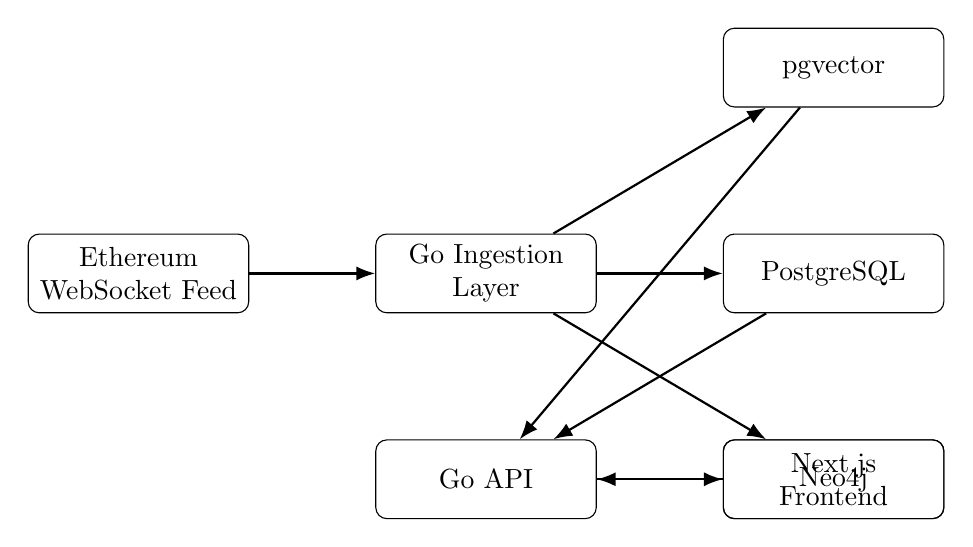
\begin{tikzpicture}[
  node distance=1.6cm and 1.6cm,
  box/.style={draw, rounded corners, align=center, minimum width=2.8cm, minimum height=1cm},
  arr/.style={-{Latex[length=2.4mm]}, thick}
]
\node[box] (eth) {Ethereum\\WebSocket Feed};
\node[box, right=of eth] (ing) {Go Ingestion\\Layer};
\node[box, right=of ing] (pg) {PostgreSQL};
\node[box, below=of pg] (neo) {Neo4j};
\node[box, above=of pg] (vec) {pgvector};
\node[box, below=of ing] (api) {Go API};
\node[box, right=of api] (web) {Next.js\\Frontend};

\draw[arr] (eth) -- (ing);
\draw[arr] (ing) -- (pg);
\draw[arr] (ing) -- (neo);
\draw[arr] (ing) -- (vec);
\draw[arr] (pg) -- (api);
\draw[arr] (neo) -- (api);
\draw[arr] (vec) -- (api);
\draw[arr] (api) -- (web);
\end{tikzpicture}
\caption{High-level system architecture.}
\end{figure}

\subsection{Implementation Overview}

\begin{tabularx}{\textwidth}{@{}p{0.18\textwidth}p{0.26\textwidth}Y@{}}
\toprule
\textbf{Layer} & \textbf{Main responsibility} & \textbf{Main implementation} \\
\midrule
Ingestion & Reads Ethereum activity and writes the source-of-truth transaction record first & \path{main.go}, \path{ingestion/worker_pool.go}, \path{client/eth.go} \\
Relational store & Accounts, transactions, flags, metadata, enrichment queue & \path{store/postgres.go} \\
Graph store & Graph neighborhoods, traces, hubs, circular flows & \path{store/neo4j.go} \\
Vector search & Contract and account similarity & \path{store/vector.go} \\
API & Backend routes consumed by the frontend & \path{api/server.go} \\
Frontend & Overview, account, graph, transaction, and contract pages & \path{web/app/} \\
\bottomrule
\end{tabularx}

\subsection{Current Product Surfaces}

\begin{itemize}
\item \textbf{Overview}: summary metrics, transaction history, recent flags, recent transactions
\item \textbf{Account profile}: account summary, counterparties, recent transactions, behavior similarity, velocity chart
\item \textbf{Graph workspace}: hop-based tracing, center-node fallback, hub list, path tracing
\item \textbf{Transaction detail}: ledger event view with counterparties, payload, and linked flags
\item \textbf{Contract analysis}: recent contracts, contract detail, bytecode-based similarity
\end{itemize}

\subsection{Design Decisions}

\begin{itemize}
\item PostgreSQL is written first, then graph and vector enrichment run asynchronously.
\item Neo4j is a specialized secondary store for path and connectivity queries.
\item pgvector stays inside PostgreSQL instead of introducing a fourth service.
\item A seeded known-entity catalog improves interpretability without replacing live data.
\end{itemize}

\section{Current Backlog}

\begin{itemize}
\item richer known-entity coverage
\item better contract metadata ingestion
\item watchlists and saved searches
\item improved graph cluster views
\item authentication and role-based access control
\item more automated tests and benchmarking
\end{itemize}

\section{Database Schema (E-R Diagram, Keys, and Descriptions)}

\subsection{Why Multiple Databases Were Used}

\begin{tabularx}{\textwidth}{@{}p{0.22\textwidth}Y@{}}
\toprule
\textbf{Technology} & \textbf{Why it was used} \\
\midrule
PostgreSQL & transactional integrity, foreign keys, constraints, metrics, and source-of-truth storage \\
Neo4j & pathfinding, neighborhood expansion, hubs, and circular-flow queries \\
pgvector & nearest-neighbor search for contracts and behavioral profiles \\
\bottomrule
\end{tabularx}

\subsection{PostgreSQL E-R Diagram}

\begin{figure}[h]
\centering
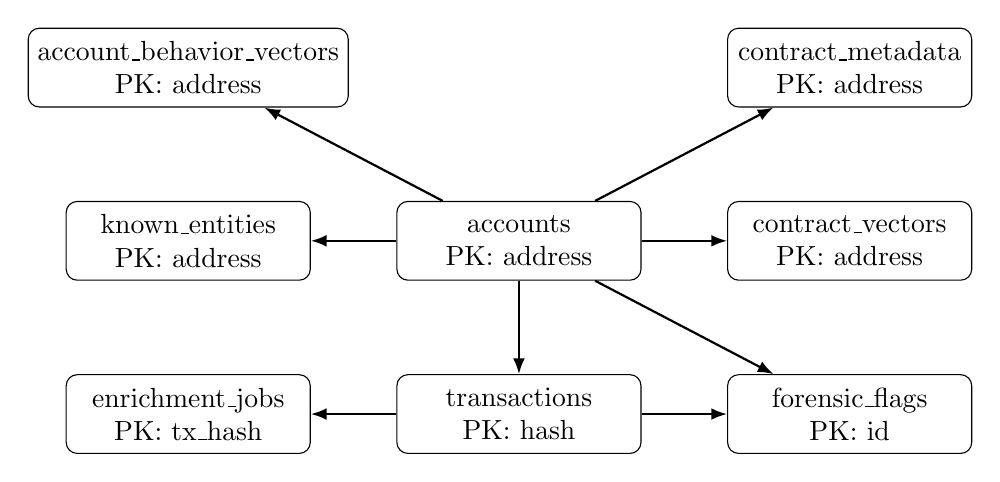
\begin{tikzpicture}[
  entity/.style={draw, rounded corners, align=center, minimum width=3.1cm, minimum height=1cm},
  rel/.style={-{Latex[length=2mm]}, thick}
]
\node[entity] (accounts) at (0,0) {accounts\\PK: address};
\node[entity] (tx) at (0,-2.2) {transactions\\PK: hash};
\node[entity] (flags) at (4.2,-2.2) {forensic\_flags\\PK: id};
\node[entity] (jobs) at (-4.2,-2.2) {enrichment\_jobs\\PK: tx\_hash};
\node[entity] (known) at (-4.2,0) {known\_entities\\PK: address};
\node[entity] (cv) at (4.2,0) {contract\_vectors\\PK: address};
\node[entity] (cm) at (4.2,2.2) {contract\_metadata\\PK: address};
\node[entity] (abv) at (-4.2,2.2) {account\_behavior\_vectors\\PK: address};

\draw[rel] (accounts) -- (tx);
\draw[rel] (accounts) -- (flags);
\draw[rel] (tx) -- (flags);
\draw[rel] (tx) -- (jobs);
\draw[rel] (accounts) -- (known);
\draw[rel] (accounts) -- (cv);
\draw[rel] (accounts) -- (cm);
\draw[rel] (accounts) -- (abv);
\end{tikzpicture}
\caption{Core PostgreSQL relations used by the submitted application.}
\end{figure}

\subsection{Table Descriptions and Keys}

\begin{tabularx}{\textwidth}{@{}p{0.24\textwidth}p{0.14\textwidth}Y@{}}
\toprule
\textbf{Table} & \textbf{Primary key} & \textbf{Important foreign keys / notes} \\
\midrule
\path{accounts} & \path{address} & parent relation for observed Ethereum addresses \\
\path{transactions} & \path{hash} & \path{from_address -> accounts.address}, \path{to_address -> accounts.address} \\
\path{forensic_flags} & \path{id} & \path{tx_hash -> transactions.hash}, \path{address -> accounts.address} \\
\path{enrichment_jobs} & \path{tx_hash} & \path{tx_hash -> transactions.hash}; durable queue model \\
\path{known_entities} & \path{address} & \path{address -> accounts.address}; seeded labels \\
\path{contract_vectors} & \path{address} & \path{address -> accounts.address}; stores bytecode and embeddings \\
\path{contract_metadata} & \path{address} & \path{address -> accounts.address}; ABI stored as \path{JSONB} \\
\path{account_behavior_vectors} & \path{address} & \path{address -> accounts.address}; behavior embedding and features \\
\bottomrule
\end{tabularx}

\subsection{Design Quality}

\begin{itemize}
\item the relational core is normalized around \path{accounts}, \path{transactions}, and \path{forensic_flags}
\item PostgreSQL transactions provide ACID guarantees on the primary write path
\item Neo4j and pgvector are enrichment layers, so the full multi-store system is eventually consistent outside PostgreSQL
\item \path{JSONB} is used only where semi-structured data is justified, especially contract ABI and behavior features
\end{itemize}

\section{Links to Code}

\begin{itemize}
\item \path{main.go}
\item \path{client/eth.go}
\item \path{ingestion/worker_pool.go}
\item \path{store/postgres.go}
\item \path{store/neo4j.go}
\item \path{store/vector.go}
\item \path{forensics/circular.go}
\item \path{forensics/anomaly.go}
\item \path{api/server.go}
\item \path{web/app/overview/page.tsx}
\item \path{web/app/accounts/[address]/page.tsx}
\item \path{web/app/graph/page.tsx}
\item \path{web/app/transactions/[hash]/page.tsx}
\item \path{web/app/contracts/page.tsx}
\item \path{web/app/contracts/[address]/page.tsx}
\end{itemize}

\section{Test Case Specifications}

\begin{tabularx}{\textwidth}{@{}p{0.08\textwidth}p{0.18\textwidth}p{0.34\textwidth}Y@{}}
\toprule
\textbf{ID} & \textbf{Area} & \textbf{Test case} & \textbf{Expected result} \\
\midrule
T1 & Backend build & Run \texttt{go build ./...} & Backend compiles \\
T2 & Frontend build & Run \texttt{pnpm build} in \path{web/} & Frontend compiles \\
T3 & Overview API & Request \texttt{GET /stats/overview} & Returns core counters \\
T4 & Account profile & Request \texttt{GET /accounts/\{address\}/profile} & Returns profile aggregates and recent transactions \\
T5 & Graph & Request \texttt{GET /addresses/\{address\}/graph} & Returns graph data or center-node fallback \\
T6 & Trace & Request \texttt{GET /addresses/\{address\}/trace?to=\{target\}} & Returns a bounded path if one exists \\
T7 & Transactions & Request \texttt{GET /transactions/\{hash\}} and \texttt{GET /transactions/\{hash\}/flags} & Returns ledger detail and related flags \\
T8 & Contracts & Request \texttt{GET /contracts/recent} and \texttt{GET /contracts/\{address\}} & Returns contract summaries and details \\
T9 & Similarity & Request \texttt{GET /contracts/\{address\}/similar} or \texttt{GET /accounts/\{address\}/similar} & Returns vector-based nearest neighbors \\
\bottomrule
\end{tabularx}

\section{Limitations and Possibilities for Improvement}

\subsection{Current Limitations}

\begin{itemize}
\item the system only covers ingested Ethereum activity, not the full chain history
\item Neo4j and pgvector can temporarily lag behind PostgreSQL
\item contract metadata depth depends on what has been populated in \path{contract_metadata}
\item similarity and forensic flags are investigative signals, not proof
\item the current product does not yet include authentication or collaboration features
\end{itemize}

\subsection{Improvements}

\begin{itemize}
\item broaden the known-entity catalog
\item ingest richer contract metadata and decoding results
\item add watchlists and saved searches
\item add role-based authentication
\item add more automated integration tests and performance measurements
\end{itemize}

\end{document}
